% Auto-generated from experiment results.
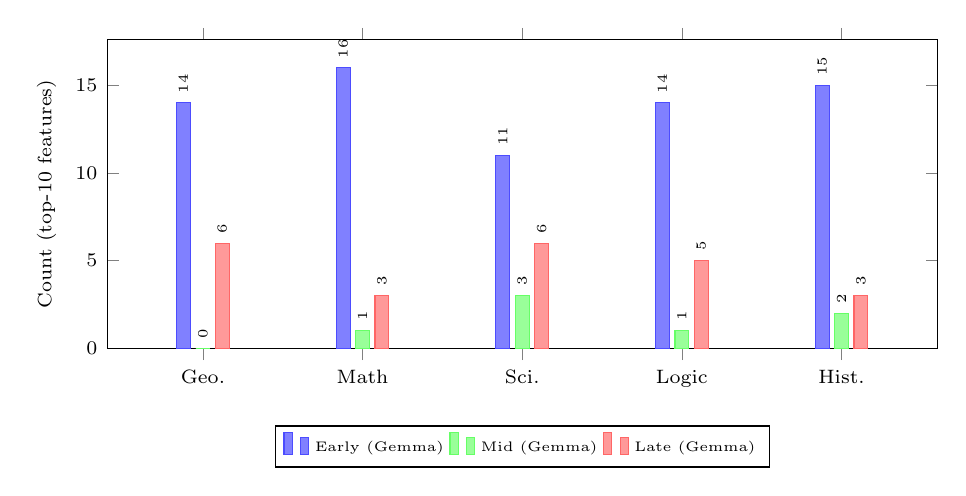
\begin{tikzpicture}
\begin{axis}[
    ybar,
    width=\columnwidth,
    height=5.5cm,
    bar width=5pt,
    ylabel={Count (top-10 features)},
    symbolic x coords={Geo., Math, Sci., Logic, Hist.},
    xtick=data,
    x tick label style={font=\scriptsize},
    y tick label style={font=\scriptsize},
    ylabel style={font=\scriptsize},
    legend style={
        font=\tiny,
        at={(0.5,-0.25)},
        anchor=north,
        legend columns=3
    },
    ymin=0,
    enlarge x limits=0.15,
    nodes near coords,
    nodes near coords style={font=\tiny, rotate=90, anchor=west},
]

\addplot[fill=blue!50, draw=blue!70] coordinates {
    (Geo., 14) (Math, 16) (Sci., 11) (Logic, 14) (Hist., 15)
};
\addplot[fill=green!40, draw=green!60] coordinates {
    (Geo., 0) (Math, 1) (Sci., 3) (Logic, 1) (Hist., 2)
};
\addplot[fill=red!40, draw=red!60] coordinates {
    (Geo., 6) (Math, 3) (Sci., 6) (Logic, 5) (Hist., 3)
};

\legend{Early (Gemma), Mid (Gemma), Late (Gemma)}

\end{axis}
\end{tikzpicture}
